\documentclass{Configuration_Files/PoliMi3i_thesis}

% CONFIGURATIONS
\usepackage{parskip} % For paragraph layout
\usepackage{setspace} % For using single or double spacing
\usepackage{emptypage} % To insert empty pages
\usepackage{multicol} % To write in multiple columns (executive summary)
\setlength\columnsep{15pt} % Column separation in executive summary
\setlength\parindent{0pt} % Indentation
\raggedbottom  

% PACKAGES FOR TITLES
\usepackage{titlesec}
% \titlespacing{\section}{left spacing}{before spacing}{after spacing}
\titlespacing{\section}{0pt}{3.3ex}{2ex}
\titlespacing{\subsection}{0pt}{3.3ex}{1.65ex}
\titlespacing{\subsubsection}{0pt}{3.3ex}{1ex}
\usepackage{color}

% PACKAGES FOR LANGUAGE AND FONT
\usepackage[english]{babel} % The document is in English  
\usepackage[utf8]{inputenc} % UTF8 encoding
\usepackage[T1]{fontenc} % Font encoding
\usepackage[11pt]{moresize} % Big fonts

% PACKAGES FOR IMAGES 
\usepackage{graphicx}
\usepackage{transparent} % Enables transparent images
\usepackage{eso-pic} % For the background picture on the title page
\usepackage{subfig} % Numbered and caption subfigures using \subfloat.
\usepackage{tikz} % A package for high-quality hand-made figures.
\usetikzlibrary{}
\graphicspath{{./Images/}} % Directory of the images
\usepackage{caption} % Coloured captions
\usepackage{xcolor} % Coloured captions
\usepackage{amsthm,thmtools,xcolor} % Coloured "Theorem"
\usepackage{float}

% STANDARD MATH PACKAGES
\usepackage{amsmath}
\usepackage{amsthm}
\usepackage{amssymb}
\usepackage{amsfonts}
\usepackage{bm}
\usepackage[overload]{empheq} % For braced-style systems of equations.
\usepackage{fix-cm} % To override original LaTeX restrictions on sizes

% PACKAGES FOR TABLES
\usepackage{tabularx}
\usepackage{longtable} % Tables that can span several pages
\usepackage{colortbl}

% PACKAGES FOR ALGORITHMS (PSEUDO-CODE)
\usepackage{algorithm}
\usepackage{algorithmic}

% PACKAGES FOR REFERENCES & BIBLIOGRAPHY
\usepackage[
	colorlinks=true,
	linkcolor=black,
	anchorcolor=black,
	citecolor=black,
	filecolor=black,
	menucolor=black,
	runcolor=black,
	urlcolor=black
]{hyperref} % Adds clickable links at references
\usepackage{cleveref}
\usepackage[square, numbers, sort&compress]{natbib} % Square brackets, citing references with numbers, citations sorted by appearance in the text and compressed
\bibliographystyle{abbrvnat} % You may use a different style adapted to your field

% OTHER PACKAGES
\usepackage{pdfpages} % To include a pdf file
\usepackage{afterpage}
\usepackage{lipsum} % Dummy package
\usepackage{fancyhdr} % For the headers
\usepackage{enumitem}
\fancyhf{}
\usepackage{listingsutf8}
\usepackage{xcolor}
\usepackage{minted}

% Input of configuration file. Do not change config.tex file unless you really know what you are doing. 
% Define blue color typical of polimi
\definecolor{bluepoli}{cmyk}{0.4,0.1,0,0.4}

% Custom theorem environments
\declaretheoremstyle[
  headfont=\color{bluepoli}\normalfont\bfseries,
  bodyfont=\color{black}\normalfont\itshape,
]{colored}

% Set-up caption colors
\captionsetup[figure]{labelfont={color=bluepoli}} % Set colour of the captions
\captionsetup[table]{labelfont={color=bluepoli}} % Set colour of the captions
\captionsetup[algorithm]{labelfont={color=bluepoli}} % Set colour of the captions

\theoremstyle{colored}
\newtheorem{theorem}{Theorem}[chapter]
\newtheorem{proposition}{Proposition}[chapter]

% Enhances the features of the standard "table" and "tabular" environments.
\newcommand\T{\rule{0pt}{2.6ex}}
\newcommand\B{\rule[-1.2ex]{0pt}{0pt}}

% Pseudo-code algorithm descriptions.
\newcounter{algsubstate}
\renewcommand{\thealgsubstate}{\alph{algsubstate}}
\newenvironment{algsubstates}
  {\setcounter{algsubstate}{0}%
   \renewcommand{\STATE}{%
     \stepcounter{algsubstate}%
     \Statex {\small\thealgsubstate:}\space}}
  {}

% New font size
\newcommand\numfontsize{\@setfontsize\Huge{200}{60}}

% Title format: chapter
\titleformat{\chapter}[hang]{
\fontsize{50}{20}\selectfont\bfseries\filright}{\textcolor{bluepoli} \thechapter\hsp\hspace{2mm}\textcolor{bluepoli}{|   }\hsp}{0pt}{\huge\bfseries \textcolor{bluepoli}
}

% Title format: section
\titleformat{\section}
{\color{bluepoli}\normalfont\Large\bfseries}
{\color{bluepoli}\thesection.}{1em}{}

% Title format: subsection
\titleformat{\subsection}
{\color{bluepoli}\normalfont\large\bfseries}
{\color{bluepoli}\thesubsection.}{1em}{}

% Title format: subsubsection
\titleformat{\subsubsection}
{\color{bluepoli}\normalfont\large\bfseries}
{\color{bluepoli}\thesubsubsection.}{1em}{}

% Shortening for setting no horizontal-spacing
\newcommand{\hsp}{\hspace{0pt}}

\makeatletter
% Renewcommand: cleardoublepage including the background pic
\let\cleardoublepage\clearpage

%For correctly numbering algorithms
\numberwithin{algorithm}{chapter}

%----------------------------------------------------------------------------
%	BEGIN OF YOUR DOCUMENT
%----------------------------------------------------------------------------

\begin{document}

\fancypagestyle{plain}{%
\fancyhf{} % Clear all header and footer fields
\fancyhead[RO,RE]{\thepage} %RO=right odd, RE=right even
\renewcommand{\headrulewidth}{0pt}
\renewcommand{\footrulewidth}{0pt}}

%----------------------------------------------------------------------------
%	TITLE PAGE
%----------------------------------------------------------------------------

\pagestyle{empty} % No page numbers
\frontmatter % Use roman page numbering style (i, ii, iii, iv...) for the preamble pages

\puttitle{
	title={Low-Cost IoT System for\\Forklift Tracking and Monitoring},% Title of the thesis
	course={Internet of Things},
	name1={Kevin Ziroldi - 10764177},
	name2={Matteo Volpari - 10773593},
	advisors= {Alessandro Redondi, Fabio Palmese, Antonio Boiano}, % Supervisor name
	academicyear={2024-2025},  % Academic Year
	version={1.0}, 
	releasedate={25-5-2025}
} 
          
%----------------------------------------------------------------------------
%	PREAMBLE PAGES: ABSTRACT (inglese e italiano), EXECUTIVE SUMMARY
%----------------------------------------------------------------------------
\startpreamble
\setcounter{page}{1} % Set page counter to 1

%----------------------------------------------------------------------------
%	LIST OF CONTENTS/FIGURES/TABLES/SYMBOLS
%----------------------------------------------------------------------------

% TABLE OF CONTENTS
\thispagestyle{empty}
\tableofcontents % Table of contents 
\thispagestyle{empty}
\cleardoublepage

%-------------------------------------------------------------------------
%	THESIS MAIN TEXT
%-------------------------------------------------------------------------
% In the main text of your thesis you can write the chapters in two different ways:
%
%(1) As presented in this template you can write:
%    \chapter{Title of the chapter}
%    *body of the chapter*
%
%(2) You can write your chapter in a separated .tex file and then include it in the main file with the following command:
%    \chapter{Title of the chapter}
%    \input{chapter_file.tex}
%
% Especially for long thesis, we recommend you the second option.

% The \label{...}% enables to remove the small indentation that is generated, always leave the % symbol.

\addtocontents{toc}{\vspace{2em}} % Add a gap in the Contents, for aesthetics
\mainmatter % Begin numeric (1,2,3...) page numbering

% --------------------------------------------------------------------------
% NUMBERED CHAPTERS % Regular chapters following
% --------------------------------------------------------------------------

\chapter{System design}
\label{ch:ch1}%
\section{Data}
In this chapter we answer to question EQ1, asking to find the biggest LoRa SF for
having a success rate of at least 70\% in a LoRaWAN Network with the following parameters:
\begin{itemize}
\item Carrier frequency: $CF = 868 MHz$
\item Bandwidth: $BW = 125 kHz$
\item Number of gateways: $N_{G} = 1$
\item Number of sensor nodes: $N_{S} = 50$
\item Intensity of Poisson process: $\lambda = 1 \text{ packet/minute}$
\item Success rate: $SR \geq 0.7$
\end{itemize}

We compute the payload size based on the last two digits of the leader's person code (XY), according to the formula:
\begin{equation}
L = 3 + XY \text{ Bytes}
\end{equation}
Our leader's person code is 10773593, so the payload size is:
\begin{equation}
L = 3 + 93 = 96 \text{ Bytes}
\end{equation}

\section{Maximum Spreading Factor calculation}
Since LoRaWAN uses an ALOHA-like procedure to handle channel access and
retransmissions, we compute the success rate, SR, as the ALOHA success rate:
\begin{equation}
SR = S / G = e^{-2 G} = e^{-2 N \lambda t}
\end{equation}

Thanks to this formula, we can compute the maximum airtime to have a success rate greater than 70\%.
\begin{equation}
SR \geq 0.7
\end{equation}
\begin{equation}
e^{-2 N \lambda t} \geq 0.7
\end{equation}
By applying the natural logarithm, we get:
\begin{equation}
-2 N \lambda t \geq ln(0.7)
\end{equation}
\begin{equation}
t \leq \frac{-ln(0.7)}{2 N \lambda} = \frac{-ln(0.7)}{2 \cdot 50 \cdot \frac{1}{60 \cdot 10^3 \text{ ms}}} = 214.005 \text{ ms}
\end{equation}

We now use the API offered by The Things Network at {\color{blue}\url{https://www.thethingsnetwork.org/airtime-calculator}} to find the highest SF that guarantees an airtime smaller than the value we found. We use payload size of 96 Bytes, as computed before, region EU868 and bandwidth 125 kHz. The API says that the maximum payload size for EU868 with SF from 10 to 12 is 51 Bytes; this means that we can evaluate SF values starting from 9 and lowering the SF until we find an airtime smaller than 214.005 ms.
The values of airtime corresponding to the SF are report in the following table.

\begin{table}[H]
\centering 
\begin{tabular}{| c | c |}
	\hline 
	\rowcolor{bluepoli!40}
	\textbf{Spreading Factor} & \textbf{Airtime}\T\B \\
	\hline 
	SF9 & 594.9 ms \T\B\\
	SF8  & 328.2 ms \T\B\\
	SF7 & 184.6 ms \T\B\\
	\hline
\end{tabular}
\\[10pt]
\caption{Airtime based on SF}
\end{table}

The only value of SF that leads to an airtime smaller than 214.005 ms and a success rate greater than 70\% is SF7.

\begin{figure}[H]
    \centering
    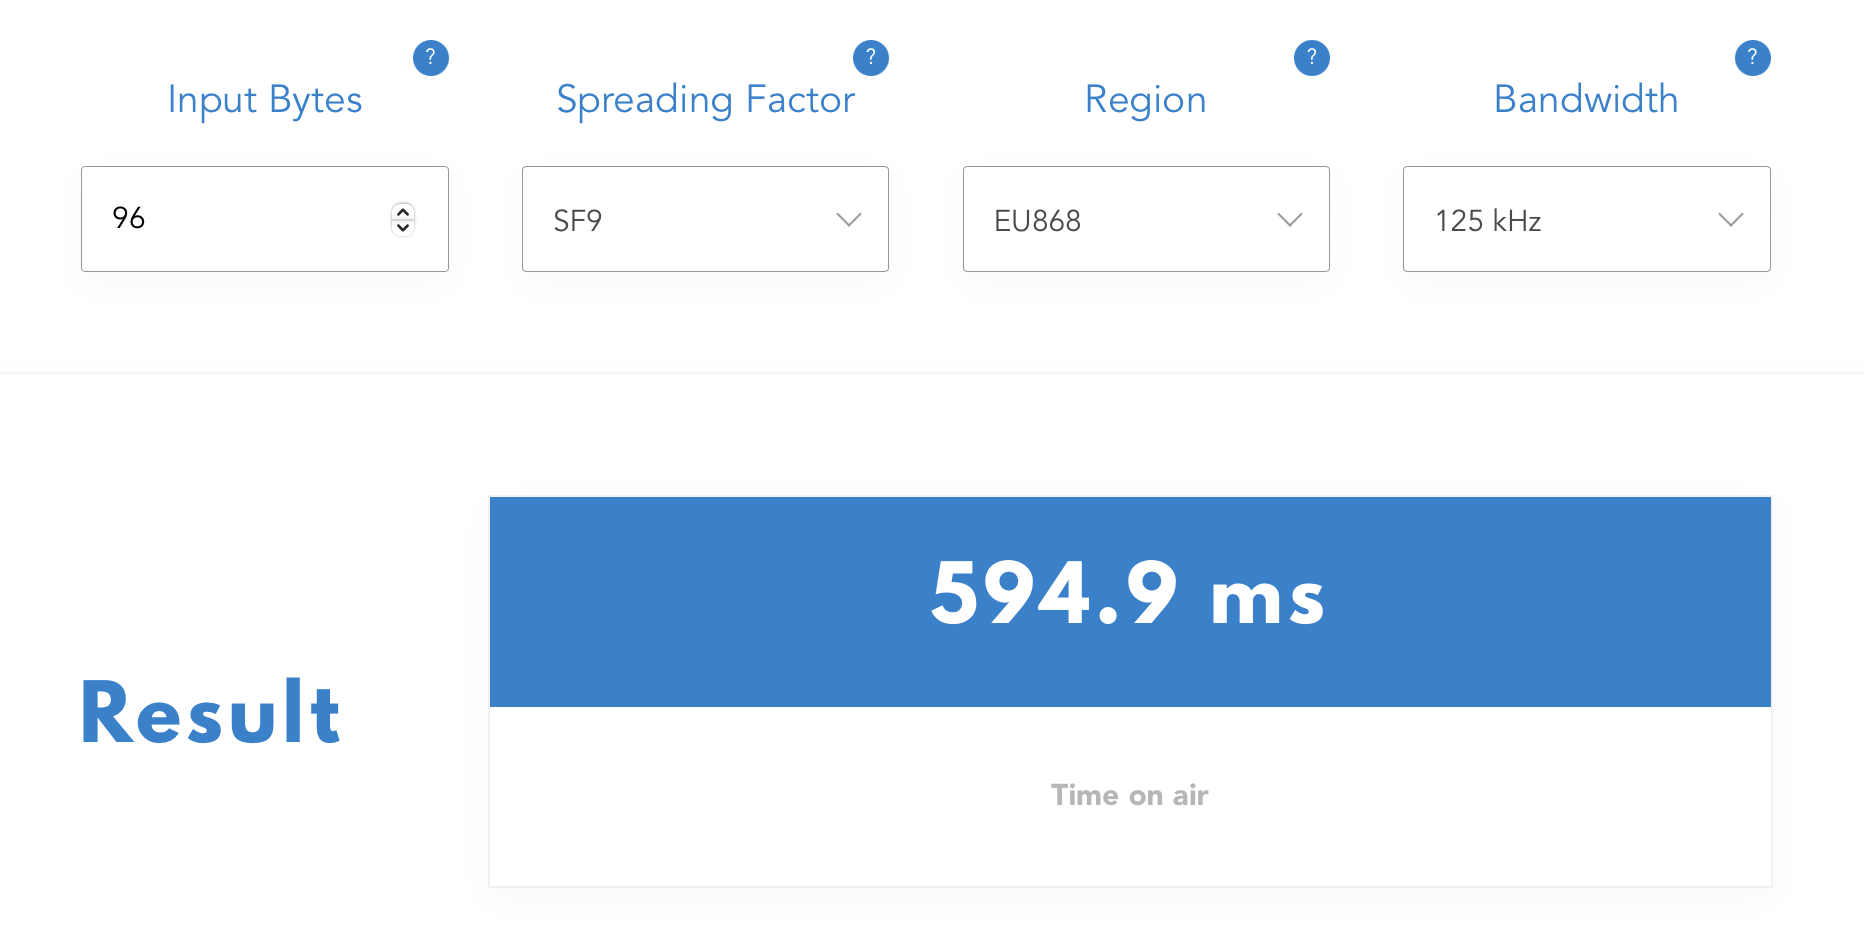
\includegraphics[width=0.6\linewidth, height=0.5\textheight, keepaspectratio]{sf9.png}
    \caption{Airtime with SF9}
\end{figure}

\begin{figure}[H]
    \centering
    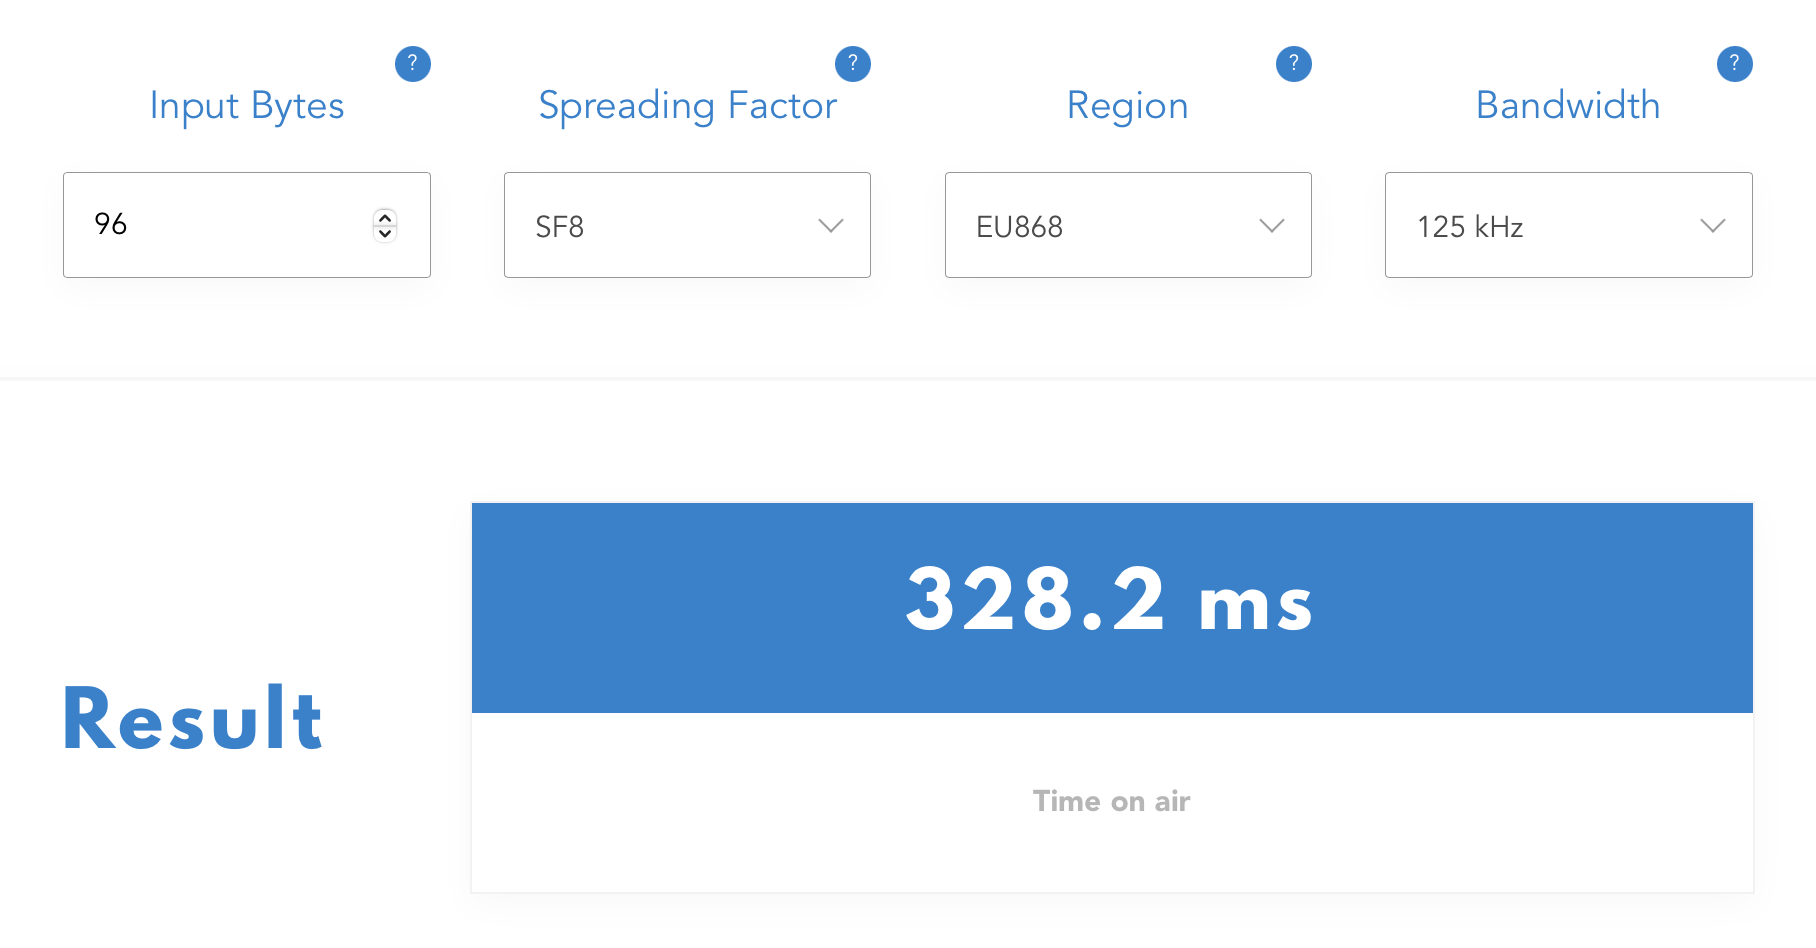
\includegraphics[width=0.6\linewidth, height=0.5\textheight, keepaspectratio]{sf8.png}
    \caption{Airtime with SF8}
\end{figure}

\begin{figure}[H]
    \centering
    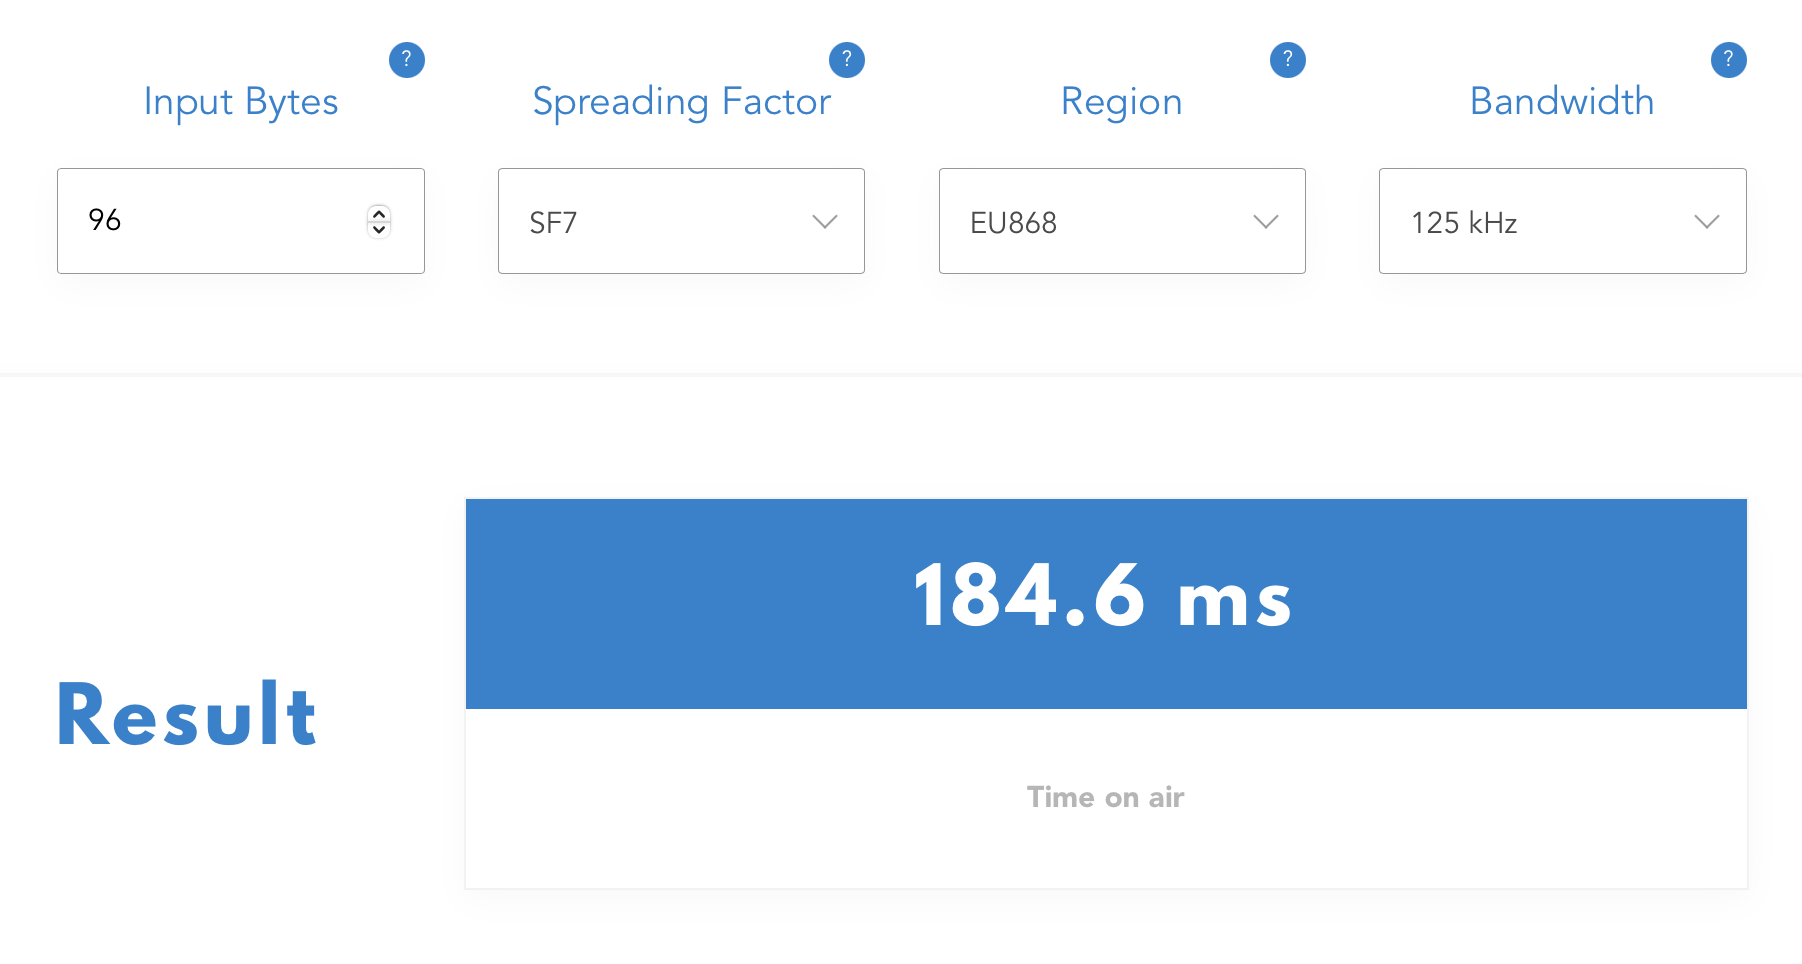
\includegraphics[width=0.6\linewidth, height=0.5\textheight, keepaspectratio]{sf7.png}
    \caption{Airtime with SF7}
\end{figure}







%-------------------------------------------------------------------------
%	BIBLIOGRAPHY
%-------------------------------------------------------------------------

\addtocontents{toc}{\vspace{2em}} % Add a gap in the Contents, for aesthetics
\bibliography{Thesis_bibliography} % The references information are stored in the file named "Thesis_bibliography.bib"

%-------------------------------------------------------------------------
%	APPENDICES
%-------------------------------------------------------------------------

% LIST OF FIGURES
%\listoffigures

% LIST OF TABLES
%\listoftables


\end{document}

